\chapter{Analysis Of Existing}

Comme dit auparavant, les flottes de drones sont régis entres elles par des modèles de mobilités. Notre étude de l'existant s'est donc décomposée en plusieurs parties.\\\\

As said before, fleets drones are governed by these models mobility. Our study of the current is therefore divided into several parts. \ \ \ \

\section{Summary of the problem}

La problématique de notre article est de scanner une zone le plus efficacement possible et le plus rapidement possible, au maximum une fois par heure. Cette zone sera scannée par une flotte de drone qui devront coopérer entre eux et communiquer.\\\\

The issue of this paper is to scan an area as efficiently as possible and as quickly as possible, at most once per hour. This area will be scanned by a fleet of drones that will cooperate and communicate.\\\\


\section{Existing models}

De nombreux modèles de mobilité existent avec chacun des caractéristiques différentes. Tous ces modèles permettent de définir des mouvements à des flottes de drones. La plupart des modèles sont basés sur des situations de la vie réelle comme la cartographie routière, ou encore sur le comportement de nombreux animaux (fourmis, oiseaux, thermites etc). Nous allons vous en exposer certains que nous considérons les plus importants et les plus intéressants pour notre cas.\\\\

Many mobility models exist each with different characteristics. All these models are used to define movements fleets drones. Most models are based on real-life situations such as road maps, or on the behavior of many animals (ants, birds, termites, wolves etc). We will expose some of which we consider the most important and most interesting for our case.\\\\ 

\subsection{Random Walk}

First described by Einstein in 1926 [29], it was developed to mimic the extremely unpredictable movement of many entities in nature [9]. An MN moves from its position to a new one by randomly choosing a direction and speed choosen by pre-defined ranges, [speedmin, speedmax] and [0, 2PI]. At the end of a constant time interval t or a constant distance traveled d, a new speed and direction are calculated. If a MN during his travel reaches a simulation boundary, it « bounces » off the simulation border with an angle determined by the incoming direction and continues to this new path.
It's a memoryless mobility pattern because it retains no knowledge of its old locations and speed values [19]. Therefore, the current position and speed of a MN is independent of its past location and speed. This can generate unrealistic movement because of sudden stops and sharp turns. If the specified time or distance of a MN motion is short, the area of the simulation will be small.

\textbf{METTRE DES SCHEMA ET DECRIRE PLUS}

\subsection{Random Waypoint}

Includes pause times between changes in direction and/or speed.Once this time expires, the MN chooses a random destination and a speed, that is uniformly distributed between [minspeed, maxspeed]. The movement pattern of a MN who uses the RWaypointMM is similar to the RwalkMM if pause time is zero and [minspeed, maxspeed] = [speedmin, speedmax].
During a performance investigation, MNs are initially distributed randomly around the simulation area. Figure 4 shows the average MN neighbor percentage of the MNs. For example, if there are 50 MNs in the network and a node has 10 neighborns, then the node's current neighbor percentage is 20\%. Moreover, during the first 600 seconds, due to initially distributed randomly of the MNs around the simulation area, there is an high variability in the average MN neighbor percentage.
In the paper, there is presented three possible solutions to avoid this initialization problem. The first is to save the location of the MNs after the initial high variability and use this position as the initial starting point of the MNs in all future simulations. Second, initially distribute the MNs in a specific area to be a distribution more common the model, like fore example, initially placing the MNs in a triangle distribution. Lastly, discard the initial 1000 seconds of simulation time in each simulation trials, to ensure thatthe initialization problem is removed even if the MNs move slowly. But if the MNs move fastly, we can discard fewer seconds of simulation time. This third solution ensures that each simulation has a random initial configuration.
Figure 5 : thre is a complex relationship between node speed and pause time. A scenario with fast MNs and long pause times actually produces a more stable networks than a scenario with slower MNs and shorter pause times. Hence, long pause times(over 20 seconds) produce a stable network even at high speeds.

\textbf{METTRE DES SCHEMA ET a revoir}

\subsection{City section}

Le but de ce modèle est de proposer un modèle réaliste. Il se base sur le mouvement de véhicule sur des cartes routières. La spécificité de ce modèle est que la carte dépend de chaque zone géographique. Ici, les véhicules sont des nœuds mobiles.
\\\\
The aim of this model is to propose a realistic model. It bases itself on the movement of vehicle on road maps. The specificity of this model is that the map depends on every geographical zone. Here, vehicles are mobile nodes.\\\\


Les données cartographique des rues sont disponibles auprès du bureau américains du recensement. Les informations concernant les cartes sont récupérées dans des fichiers textes. Ces fichiers sont composés de plusieurs éléments :
l'identifiant unique pour une route spécifiée.
la nature de la route : Cela peut être une autoroute ou une rue.
la longitude de départ.
la latitude de départ
la latitude d'arrivé.
la longitude d'arrivé.
Toutes les intersections de la carte sont représentées par des nœuds non mobile.
Ce modèle prend également en compte l'intensité du trafic routier, plus le trafic est important et plus le trait représentant la route sera gros. Ce modèle est aussi sensible à la vitesse des voitures (en fonction notamment de l'heure). Par exemple, nous pouvons considérer que la vitesse de circulation des véhicules le matin est beaucoup moins importante qu'en début d'après-midi.
Voici le déroulement de ce modèle. Chaque nœud commence à un point choisi aléatoirement et sa destination est également choisie aléatoirement. La stratégie de chaque nœud est de rechercher le plus court chemin jusqu'à la destination. Pour accomplir cela, l'algorithme de Dijkstra est utilisé. Plusieurs paramètres rentrent en compte dans cette algorithme comme la vitesse, le trafic. Ce trajet peut être changé dynamiquement. Quand un nœud a atteint sa destination, il recommence tout le processus décrit précédemment. Concernant la vitesse du nœud, il est limité à plus ou moins 5\% de la vitesse inscrite dans le fichier.\\\\


The mapping data blocks are available from the office Americans of the census. The map information is retrieved from text files. These files are composed of several elements:
\begin{itemize}
\item The unique identifier for a specified road.
\item The nature of the road: it can be a highway or a street.
\item The longitude of the start of position.
\item The latitude of the start of departure
\item The latitude of arrived.
\item The longitude of arrived.
\end{itemize}

All the intersections of the map are represented by nodes not mobile.
\textbf{This model also takes into account the volume of road traffic, the more the traffic is important and the more the line(feature) representing the road will be big. ???}
This model is also sensitive at the speed of cars (depending in particular on the hour). For example, we can consider that the speed of vehicular traffic in the morning is much smaller than at the beginning of the afternoon.
\\\\
Here is the progress of this model. Every node begins in a point chosen randomly and its destination is chosen also randomly. The strategy of every node is to look for the shortest way until the destination. To achieve it, the algorithm of Dijkstra is used. Several parameters bring in in account in this algorithm as the speed, the traffic. This route can be dynamically changed. When a node reached its destination, it begins again all the process described previously. Concerning the speed of the node, it is limited to more or less 5\% of the speed registered in the file.
\\
For example, here is a representation of the model. We see here that the traffic is little sparse, but with very different speeds.

\begin{center}
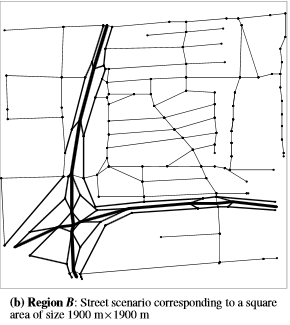
\includegraphics[width=7cm,height=50mm]{../images/city.png}
\end{center}



\textbf{METTRE DES SCHEMA ET a compléter}

\subsection{Natural Agent}

\subsubsection{Ants}

Le modèle de mobilité des fourmis se base sur le fait que les fourmis construisent des réseaux de sentiers qui relient leurs   nids avec des sources de nourritures disponible.
Chaque fourmi qui se nourrit à le même programme :

\begin{itemize}
\item Elle doit éviter les obstacles.
\item Aller ou elle veut (déplacement aléatoire) tant qu'il n'y a pas de phéromones.
\item Si elle arrive à trouver de la nourriture, elle laisse des phéromones pendant un temps t pour pouvoir indiquer aux autres fourmis l'emplacement de la nourriture.
\item Si la fourmi trouve de la nourriture, elle l'a ramène à son nid.
\end{itemize}

Les fourmis peuvent mourir. Soit elles ne trouvent pas de la nourriture assez rapidement et meurt de faim, soit elles se font tuer par d'autres prédateurs.
Tous les chemins de phéromones conduisent à de la nourriture. Mais les phéromones s'évaporent dans le temps. Le taux de phéromone peut être renforcé si plusieurs fourmis passent par le même chemin.

\textbf{METTRE DES SCHEMA ET a compléter}

\subsubsection{Termites}

\subsubsection{Wasps}

le modèle basé sur les guêpes est composé de plusieurs caractéristiques :
\begin{itemize}
\item un chef qui répartit les différentes guêpes dans différents groupes
\item 
\end{itemize}

\subsection{Birds and Fish}

\subsection{Wolves}

 